\pagenumbering{Roman}
\clearpage
\addcontentsline{toc}{section}{\protect\numberline{}Eidesstattliche Erklärung}
\section*{Eidesstattliche Erklärung}
\label{erklaerung}

Hiermit versichern wir, die vorliegende Abschlussarbeit selbstständig und nur 
unter Verwendung der von uns angegebenen Quellen und Hilfsmittel verfasst zu 
haben. Sowohl inhaltlich als auch wörtlich entnommene Inhalte wurden als 
solche kenntlich gemacht. Die Arbeit hat in dieser oder vergleichbarer Form 
noch keinem anderem Prüfungsgremium vorgelegen. \\
\\[1.5cm]
\textbf{Datum:}	12.12.2014~~~~~~~~~~~~~~~~~~~~~~~~~~~~~~~~\textbf{Unterschrift:} Andriu Maissen
\\[1.5cm]
\textbf{Datum:}	12.12.2014~~~~~~~~~~~~~~~~~~~~~~~~~~~~~~~~\textbf{Unterschrift:} Daniel Mathis
\\[1.5cm]
\textbf{Datum:}	12.12.2014~~~~~~~~~~~~~~~~~~~~~~~~~~~~~~~~\textbf{Unterschrift:} Daniel Winz
\\[1.5cm]
\textbf{Datum:}	12.12.2014~~~~~~~~~~~~~~~~~~~~~~~~~~~~~~~~\textbf{Unterschrift:} Kevin Wespi
\\[1.5cm]
\textbf{Datum:}	12.12.2014~~~~~~~~~~~~~~~~~~~~~~~~~~~~~~~~\textbf{Unterschrift:} Simon Neidhart
\\[1.5cm]
\textbf{Datum:}	12.12.2014~~~~~~~~~~~~~~~~~~~~~~~~~~~~~~~~\textbf{Unterschrift:} Yannik Küng

\clearpage
\addcontentsline{toc}{section}{\protect\numberline{}Abstract}
\section*{Abstract}
Nachfolgende Dokumentation soll eine Übersicht über die im ersten Semester geleistete Arbeit verschaffen. Anhand der Dokumentation soll aufgezeigt werden wie vorgegangen wurde um die Ziele zu erreichen. Anhand der Aufgabenstellung wurden die Projekt- und Produktanforderungen, sowie die gruppenspezifischen Ziele definiert. In einem ersten Schritt wurde eine Technologierecherche gemacht. Ziel dieser Recherche war es, bereits vorhandene Technologien zu finden. Es wurde vorwiegend im Internet auf Youtube, Wikipedia oder in Internetforen recherchiert. Anhand dieser Recherchen wurden 3 Lösungskonzepte entwickelt, ein Flugobjekt (Quadcopter), ein Bodenobjekt fahrend und ein Bodenobjekt stehend (Drehturm). Anhand von verschiedenen Tests, Berechnungen und Risikoanalysen haben wir uns für die Variante Bodenobjekt stehend (Drehturm) entschieden. Anhand der im ersten Semester geleisteten Arbeit sollte die Herstellung des Gerätes im zweiten Semester gelingen.\\
Eine weitere Möglichkeit fürs Abstract.. Im oberen sind etwas viele "{}anhand{}" drin..\\
Die Aufgabe im Modul PREN1 besteht darin ein Konzept für einen Roboter zu entwickeln. Der Roboter soll autonom 5 Bälle in einen Korb, auf einem definierten Spielfeld, befördern. Es sollten verschiedene Konzepte und Lösungswege erarbeitet werden um eine optimale Kombination herauszuarbeiten. Um eine Grundlage zu schaffen, wurden in einem Brainstorming Ideen die zu einer Lösung führen zusammengetragen. Geeignete Ansätze wurden herausgefiltert und in einem weiteren Schritt ausgearbeitet und analysiert. Anhand der Ergebnisse wurden drei Lösungskonzepte ausgewählt. Ein fliegender Roboter, einer fahrend und einer stehend. Anhand von weiteren Risikoanalysen, Berechnungen und Teilfunktionsmustern ist man zum Schluss gekommen das ein stehender Roboter die effektivste und schnellste Lösung ist um die verlangte Problemstellung zu lösen. Mit dem finalen Konzept des stehenden Roboters wurde ein für uns geeignete Strategie gewählt, welche im PREN2 die erfolgreiche Umsetzung garantieren wird.

\clearpage
\tableofcontents
\clearpage
\pagenumbering{arabic}
\section{Projektmanagement}
Das Modul PREN ist ein interdisziplinäres Modul. Von jeder der Fachrichtungen 
Informatik, Elektrotechnik und Maschinenbau ist mindestens eine Person pro 
Gruppe vertreten. Das Team 27 setzt sich wie folgt zusammen:
\begin{itemize}
    \item 3 Informatiker
    \item 3 Maschinenbauer
    \item 1 Elektrotechniker
\end{itemize}
Zu Beginn des Moduls wurden den Mitgliedern des Teams verschiedene Funktionen 
zugewiesen, um eine Struktur und somit Ansprechpersonen innerhalb des Teams zu 
erhalten. Ersichtlich ist dies in folgendem Organigramm:
\newcommand\orgnode[6][]{
    \node[#1] at (#2) {
        \boxed{
            \parbox{40pt} {%
                \includegraphics[width=40pt]{#3}}%
            \parbox{10pt}{\mbox{}}%  
            \parbox{\dimexpr4.0cm-30pt\relax}{
                \textbf{#4}\\
                [.4ex]\textit{#5}\\
                [.4ex]#6\\}%
        }
    };
}
\begin{figure}[h!]
    % from http://tex.stackexchange.com/questions/170154/organisation-chart-in-latex-using-tikz
    \centering
    \begin{tikzpicture}
        \orgnode
            {0,0}
            {../fig/takuonen.png}
            {Peter Kuonen}
            {Informatik}
            {Projektleiter}
        \orgnode
            {-6,-4}
            {../fig/tawinz.png}
            {Daniel Winz}
            {Elektrotechnik}
            {Bereichsleiter E}
        \orgnode
            {0,-4}
            {../fig/mamaisse.png}
            {Andriu Maissen}
            {Maschinenbau}
            {Bereichsleiter M}
        \orgnode
            {6,-4}
            {../fig/taneidha.png}
            {Simon Neidhart}
            {Informatik}
            {Bereichsleiter I}
        \orgnode
            {0,-8}
            {../fig/tfkueng.png}
            {Yannik Küng}
            {Maschinenbau}
            {Projektmitarbeiter}
        \orgnode
            {0,-12}
            {../fig/tfmathis.png}
            {Daniel Mathis}
            {Maschinenbau}
            {Projektmitarbeiter}
        \orgnode
            {6,-8}
            {../fig/tcwespi.png}
            {Kevin Wespi}
            {Informatik}
            {Protokollführer}
        \draw[-latex, thick] (0,-1) -- (0,-2) -- (-6,-2) -- (-6,-3);
        \draw[-latex, thick] (0,-1) -- (0,-2) -- (0,-2) -- (0,-3);
        \draw[-latex, thick] (0,-1) -- (0,-2) -- (6,-2) -- (6,-3);
        \draw[-latex, thick] (-2.4,-4) -- (-2.9,-4) -- (-2.9,-8) -- (-2.4, -8);
        \draw[-latex, thick] (-2.4,-4) -- (-2.9,-4) -- (-2.9,-12) -- (-2.4, -12);
        \draw[-latex, thick] (3.6,-4) -- (3.1,-4) -- (3.1,-8) -- (3.6, -8);
    \end{tikzpicture}
    \caption{Organigramm}
    \label{fig:Organigramm}
\end{figure}

\subsection{Projektplanung}
In den folgenden Abbildungen wird die Planung mittels Zeitachsen für die 
einzelnen Meilensteine dargestellt. Sie enthalten die Hauptaufgaben, welche 
für die jeweiligen Meilensteine notwendig sind. Die Planung wird angefertigt 
um die Übersicht über das Projekt zu haben und die verlangten Dokumente und 
Schritte zur Erfüllung der Meilensteine fristgerecht zu erledigen.

\begin{figure}[h!]
    \centering
    \begin{tikzpicture}[scale=0.5]
        % Phases
        \draw[fill=lgray, align=center, rounded corners] (0,- 0) rectangle node {Moduleinführung\\Teambildung\\Projektinitialisierung} (-8,- 8);
        \draw[fill=lgray, align=center, rounded corners] (0,- 8) rectangle node {Projektplanung\\Anforderungen\\Recherche} (-8,-15);
        \draw[fill=lgray, align=center, rounded corners] (0,-15) rectangle node {Anforderungen\\Recherche} (-8,-22);
        % Days
        \draw[thick] (0,- 0) -- (1,- 0) node[right] {18.09.2014};
        \draw[thick] (0,- 1) -- (1,- 1) node[right] {19.09.2014};
        \draw[thick] (0,- 7) -- (1,- 7) node[right] {25.09.2014};
        \draw[thick] (0,- 8) -- (1,- 8) node[right] {26.09.2014};
        \draw[thick] (0,-14) -- (1,-14) node[right] {02.10.2014};
        \draw[thick] (0,-15) -- (1,-15) node[right] {03.10.2014};
        \draw[thick] (0,-21) -- (1,-21) node[right] {09.10.2014};
        \draw[thick] (0,-22) -- (1,-22) node[right] {10.10.2014};
        % Arrow
        \draw[line width=4, ->] (0,0) -- (0,-22.5);
    \end{tikzpicture}
    \caption{Planung Meilenstein 1 (Initialisierungsphase)}
    \label{fig:MS1}
\end{figure}
\begin{figure}[h!]
    \centering
    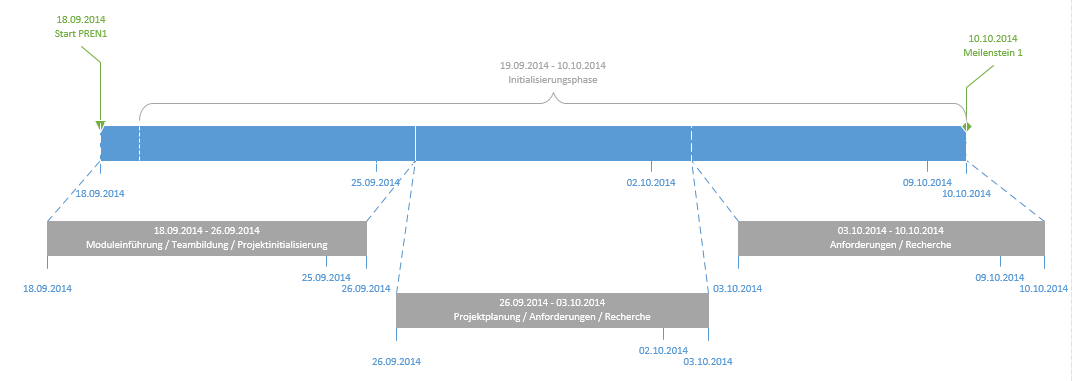
\includegraphics[angle=90,height=0.9\textheight]{fig/PlanungBisMS1.png}
    \caption{Planung Meilenstein 1}
    \label{fig:MS1}
\end{figure}
\begin{figure}[h!]
    \centering
    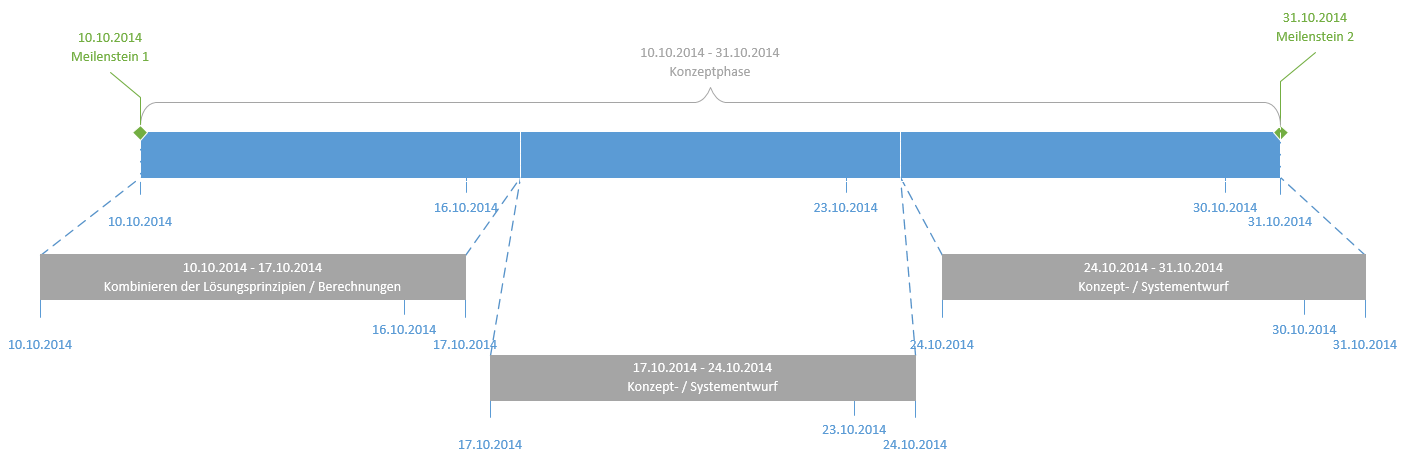
\includegraphics[angle=90,height=0.9\textheight]{fig/PlanungBisMS2.png}
    \caption{Planung Meilenstein 2}
    \label{fig:MS2}
\end{figure}
\begin{figure}[h!]
    \centering
    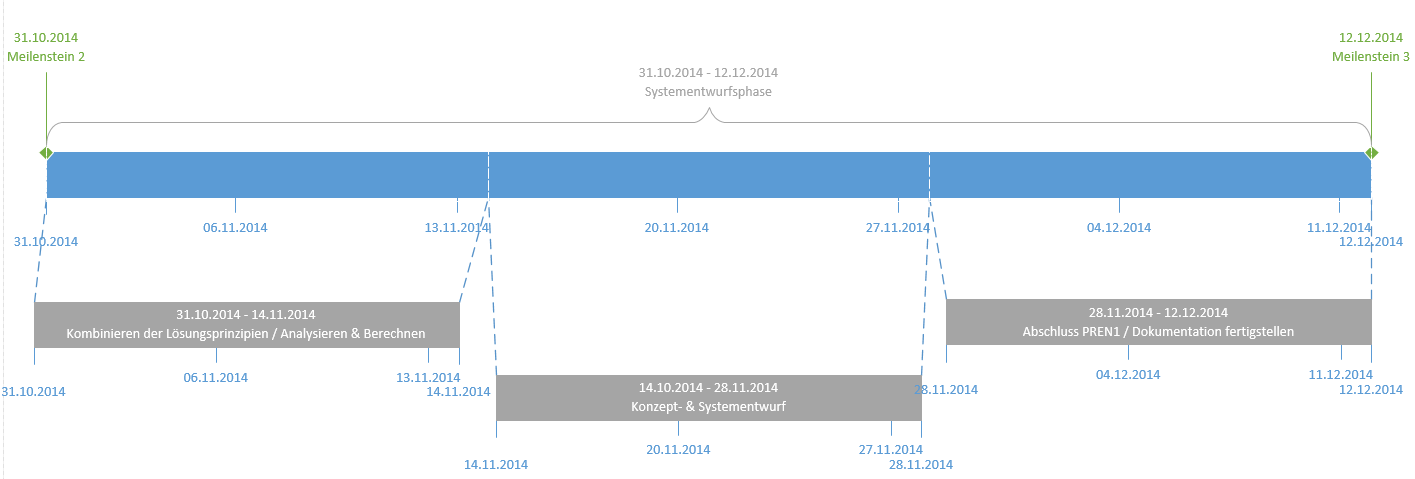
\includegraphics[angle=90,height=0.9\textheight]{fig/PlanungBisMS3.png}
    \caption{Planung Meilenstein 3}
    \label{fig:MS3}
\end{figure}

\clearpage
%\begin{landscape}

\subsection{Risikoanalyse allgemein}
Bevor das Projekt richtig gestartet wird, soll eine allgemeine Risikoanalyse erstellt werden. Das Team hat sich Gedanken darüber gemacht, was schief gehen kann und wie man mit den erkannten Problemen umgehen oder ihnen vorbeugen kann. Zudem wurde die Wahrscheinlichkeit und die Auswirkung der eruierten Probleme notiert. Mit der Liste im Hinterkopf wird das Projekt mit einem anderen Mindset angegangen und Fehlerquellen werden minimiert. 

\begin{table}[h!]
	\begin{zebratabular}{@{}cp{0.25\linewidth}llp{0.25\linewidth}}		
		\textbf{ID}&\textbf{Beschreibung}&\textbf{Wahrscheinlichkeit}&\textbf{Auswirkung}&\textbf{Massnahmen}\\
		\hline
		\#1&Teammitglied Elektrotechnik fällt aus&sehr niedrig&sehr hoch&keine\\
		\#2&Teammitglied Maschinenbau fällt aus&sehr niedrig&hoch&Übernahme durch Maschinenbauer\\
		\#3&Teammitglied Informatik fällt aus&sehr niedrig&hoch&Übernahme durch Informatiker\\
		\#4&Budget wird überschritten&niedrig&hoch&Vorab Kosten abklären\\
		\#5&Zeit reicht nicht zur Realisierung&mittel&sehr hoch&Zeitplanung mit Meilensteinen\\
		\#6&Eingekaufte Komponente fällt aus&niedrig&hoch&Neu bestellen\\
		\#7&Komponente (Eigenbau) fällt aus&niedrig&mittel&Neu bauen\\
		\#8&Komponente funktioniert nicht&niedrig&mittel&Komponente reparieren\\
		\#9&Berechnungen falsch&sehr niedrig&hoch&Überprüfung durch mehrere Personen\\
		\#10&Abmessungseinschränkungen überschritten&sehr niedrig&hoch&Modell bauen\\
		\#11&Schnittstellen ungenau definiert&sehr niedrig&sehr hoch&Überprüfung durch mehrere Personen\\
		\#12&Startsignal funktioniert nicht&niedrig&hoch&Ausgiebiges Testen\\
		\#13&Endsignal nicht übermittelt&niedrig&sehr niedrig&Ausgiebiges Testen\\
		\#14&Verfehlen des Korbs&mittel&mittel&Ausgiebiges Testen\\
		\#15&Stromversorgung reicht nicht aus&sehr niedrig&mittel&Ausgiebiges Testen\\
		\#16&Anforderungen ändern&sehr niedrig&hoch&Neu planen\\
	\end{zebratabular}
\end{table}
%\end{landscape}

\clearpage
\section{Einleitung}
Die Module PREN1 und PREN2 (Produktentwicklung) sind Teil des Studiums einer 
technischen Fachrichtung an der Hochschule Luzern Technik \& Architektur 
(HSLU T\&A). 
Zu Beginn des Moduls werden die Studierenden in interdisziplinäre Teams 
eingeteilt. Diese Teams umfassen Studierende der Studiengänge Maschinenbau, 
Informatik und Elektrotechnik. Die Teams erhalten am ersten Tag eine Aufgabe. 
Diese Aufgabe muss dann in den nächsten zwei Semestern gelöst werden. 
Die Aufgabe für das Herbst- und Frühlingssemester 2014/2015 ist es, ein Gerät
zu entwickeln, das in der Lage ist, einen Ball in einen Korb zu befördern.
Einschränkungen dabei bilden die Grösse des Spielfelds und die Bedingung, dass
die Bälle entweder geworfen oder geflogen werden müssen. 
Details, siehe Abschnitt \ref{sec:aufgabe}

\clearpage
\section{Aufgabenstellung}
\label{sec:aufgabe}
Es soll ein Gerät entwickelt werden, das Bälle in einen Korb werfen kann. 
Dies soll Autonom erfolgen. 
\begin{figure}[h!]
    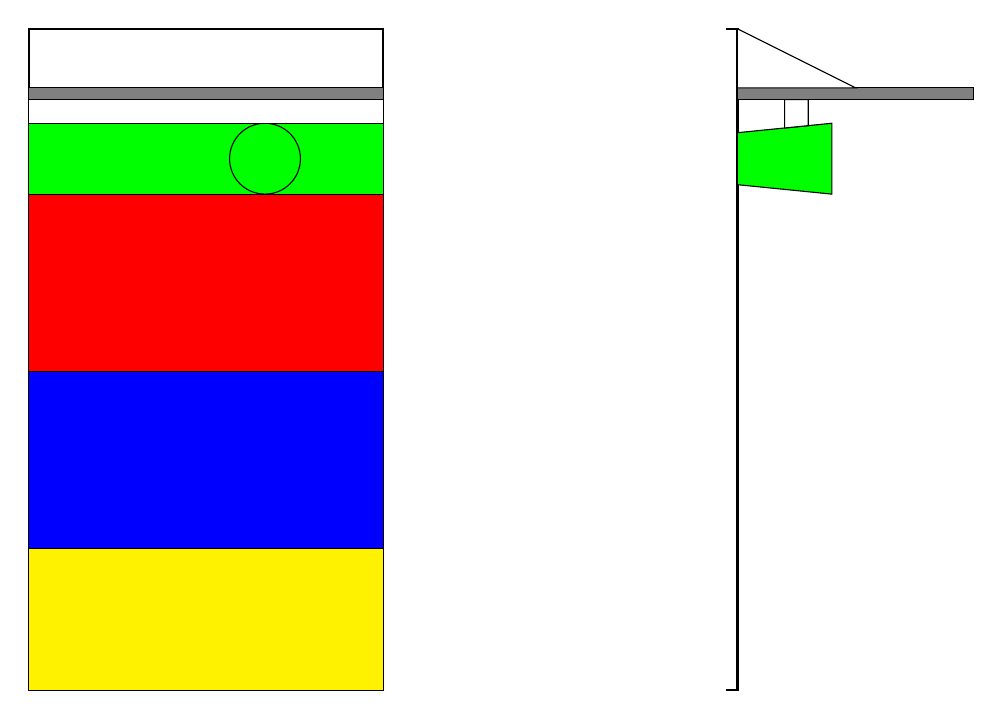
\begin{tikzpicture}[scale=0.03]
        % playfield frame
        \draw[thick] (0,0) rectangle (150,280);
        \draw[thick] (295,0) -- (300,0) -- (300,280) -- (295,280);
        % startfield
        \draw[fill=yellow] (0,0) rectangle (150,60);
        % move field
        \draw[fill=blue] (0,60) rectangle (150,135);
        % border line
        \draw[thick] (0,135) -- (150,135);
        % void field
        \draw[fill=red] (0,135) rectangle (150,210);
        % basket field
        \draw[fill=green] (0,210) rectangle (150,240);
        % basket
        \draw[fill=green] (100,225) circle [radius=15];
        \draw[fill=green] (300,214) -- (340,210) -- (340,240) -- (300,236) -- (300,214);
        % gap filler
        \draw[fill=white] (0,240) rectangle (150,250);
        \draw[fill=white] (320,250) -- (320,238) -- (330,239) -- (330,250) -- (320,250);
        % wall
        \draw[fill=gray] (0,250) rectangle (150,255);
        \draw[fill=gray] (300,250) rectangle (400,255);
        \draw[fill=white] (300,255) -- (350,255) -- (300,280) -- (300,255);
    \end{tikzpicture}
    \caption{Spielfeld}
    \label{fig:playfield}
\end{figure}

\subsection{Eigene Anforderungen}

\clearpage
\newcommand{\morphcellwidth}
{
0.12\linewidth
}
\section{Lösungskonzepte}
Mit diesem Abschnitt sollen die erarbeiteten Konzepte gegenübergestellt und 
anhand von vorgegebenen Kriterien bewertet werden. Dies ergibt eine 
Auswahl der optimalen Kombination, welche in einem nächsten Schritt 
ausgearbeitet wird. Das daraus resultierende, definitive Konzept wird im nachfolgenden Kapitel "Produktbeschreibung Funktion" näher erläutert. 
Das im Anhang beigefügte Dokument "'Brainstorming"' zeigt die ersten Ideen für 
die verschiedenen Funktionsweisen. Hierbei wurde weder auf Risiken, Kosten 
noch auf Umsetzbarkeit geachtet. In einem weiteren Schritt werden die 
sinnvollsten Kombinationen in morphologischen Kästen kombiniert und für die 
jeweiligen Lösungen erweitert und ausgewertet. 

\subsection{Distanzmessung - optische Erkennung}
Für das Erkennen des Korbs wurde auf Distanzmessung mittels Laser, Ultraschall oder 
ähnlichem verzichtet. Hauptsächlich aus dem Grund, weil von der Abteilung Informatik 
im gesamten Projekt nicht viel Programmieraufwand gefordert ist. Durch die Wahl der 
optischen Erkennung über eine Kamera ist für die Informatik eine Teilfunktion entstanden, 
die einiges an Programmieren verlangt. Aus diesem Grund wird in den folgenden 
morphologischen Kästen auf Distanzmessung als Option verzichtet und standardmässig 
optische Erkennung ausgewählt.


\subsection{Variante Bodenobjekt fahrend}
\subsubsection{Kurzbeschrieb}
Bei diesem Konzept soll die Abschussvorrichtung fahrend sein. Hierbei kann 
die  Wurfdistanz zum Ziel verringert werden und auch das Zielen mittels 
Bewegung erfolgen.

\clearpage

\subsubsection{Morphologischer Kasten}
% Morphologischer Kasten mit Stichworten
\footnotesize
\begin{table}[h!]
    \begin{zebratabular}{@{}p{0.2\linewidth}p{\morphcellwidth}p{\morphcellwidth}p{\morphcellwidth}p{\morphcellwidth}p{\morphcellwidth}p{\morphcellwidth}}
    %\begin{zebratabular}{@{}p{0.2\linewidth}llllll}
        \rowcolor{gray}
        Eigenschaften &
            \multicolumn{6}{c}{Merkmalausprägung} \\
        Art der Bewegung &
            Fliegend                \tikzmark{1move:fly}          &
            Fahrend                 \tikzmark{1move:drive}        &
            Stehend                 \tikzmark{1move:stay}         &
                                    \tikzmark{1move:none3}        &
                                    \tikzmark{1move:none2}        &
                                    \tikzmark{1move:none1}        \\
        Ballbeförderung &
            Ballistisch             \tikzmark{1ballmove:ball}     &
            Abwurf                  \tikzmark{1ballmove:drop}     &
                                    \tikzmark{1ballmove:none4}    &
                                    \tikzmark{1ballmove:none3}    &
                                    \tikzmark{1ballmove:none2}    &
                                    \tikzmark{1ballmove:none1}    \\
        Erkennen des Korbes &
            Distanzmessung          \tikzmark{1localize:dist}     &
            Optische Erkennung      \tikzmark{1localize:opt}      &
                                    \tikzmark{1localize:none4}    &
                                    \tikzmark{1localize:none3}    &
                                    \tikzmark{1localize:none2}    &
                                    \tikzmark{1localize:none1}    \\
        Balllager &
            Einzeln                 \tikzmark{1store:single}      &
            Zusammen                \tikzmark{1store:mult}        &
                                    \tikzmark{1store:none4}       &
                                    \tikzmark{1store:none4}       &
                                    \tikzmark{1store:none4}       &
                                    \tikzmark{1store:none1}       \\
        Übertragung Startsignal &
            Funk                    \tikzmark{1connect:radio}     &
            Optisch                 \tikzmark{1connect:opt}       &
            Ultraschall             \tikzmark{1connect:us}        &
            Spracherkennung         \tikzmark{1connect:voice}     &
                                    \tikzmark{1connect:none2}     &
                                    \tikzmark{1connect:none1}     \\
        Energieversorgung &
            intern elektrisch       \tikzmark{1power:elint}       &
            extern elektrisch       \tikzmark{1power:elext}       &
            Verbrennungsmotor       \tikzmark{1power:combustion}  &
            Druckluft               \tikzmark{1power:air}         &
            Potenzielle Energie     \tikzmark{1power:height}      &
            Feder                   \tikzmark{1power:spring}      \\
    \end{zebratabular}
\end{table}

% Linien zur Darstellung von Lösungsvarianten
\begin{tikzpicture}[remember picture,overlay]
    \draw [ultra thick, rounded corners, red] 
        ({pic cs:1move:drive}) circle(2pt)
        --
        ({pic cs:1ballmove:ball}) circle(2pt)
        --
        ({pic cs:1localize:opt}) circle(2pt)
        --
        ({pic cs:1store:single}) circle(2pt)
        --
        ({pic cs:1connect:radio}) circle(2pt)
        --
        ({pic cs:1power:elint}) circle(2pt)
        ;
\end{tikzpicture}
\normalsize

\subsubsection{Vor- und Nachteile}
\begin{minipage}{\textwidth}
    \begin{itemize}
    	\item[+] auffallend
    	\item[+] Distanz zum Korb ist immer gleich
    	\item[-] langsam (lange Ausrichtzeit)
    	\item[-] aufwändige Konstruktion
    	\item[-] hohes Gewicht
    \end{itemize}
\end{minipage}

\subsubsection{Funktionsweise}
Eine fahrende Lösung wäre durch das anfängliche Ausrichten des Geräts und 
den anschliessenden Wurf ein technisch anspruchsvoller und interessanter 
Ansatz. Jedoch wird gerade aufgrund dieser Punkte das Erreichen der 
Projektziele erschwert. Das Fahren benötigt im Vergleich zu einem direkten 
Wurf, welcher durch die kurze Distanz gut realisierbar ist, viel Zeit. Auch 
wird die Konstruktion durch die Fortbewegung komplizierter und somit 
teurer und schwerer. Durch die klare Aufgabenstellung ist eine 
universellere Nutzung mit eventuellen Erweiterungsmöglichkeiten nicht nötig. 

\subsubsection{Risikoanalyse Konzept 1 (Bodenobjekt fahrend)}
\begin{table}[h!]
	\begin{zebratabular}{@{}cp{0.25\linewidth}llp{0.25\linewidth}}		
		\textbf{ID}&\textbf{Beschreibung}&\textbf{Wahrscheinlichkeit}&\textbf{Auswirkung}&\textbf{Massnahmen}\\
		\hline
		\#17&Fahrmechanismus funktioniert nicht&niedrig&hoch&Ausgiebiges Testen\\
		\#18&Ausrichten funktioniert nicht&niedrig&sehr hoch&Ausgiebiges Testen\\
		\#19&Balllager (Nachschieben) streikt&sehr niedrig&hoch&Mechanismus einbauen, der nicht blockiert\\
		\#20&Umfallen durch Rückstoss&sehr niedrig&niedrig&Ausgiebiges Testen\\		
	\end{zebratabular}
\end{table}


\clearpage

\subsection{Variante Flugobjekt}
\subsubsection{Kurzbeschrieb}
Mit der Wahl eines fliegenden Objektes kann viel Aufsehen erregt werden. 
Allerdings gestaltet sich die Konstruktion auch schwieriger als bei anderen 
Geräten. Ebenfalls ein wichtiger Faktor ist die Herausforderung für die Gruppe 
erfolgreich ein fliegendes Objekt zu bauen. Da im Handel schon 
unterschiedliche Flugobjekte preiswert erworben werden können, scheint die 
Aufgabe einfacher, als dass sie es wirklich ist.

\subsubsection{Morphologischer Kasten}
% Morphologischer Kasten mit Stichworten
\footnotesize
\begin{table}[h!]
    \begin{zebratabular}{@{}p{0.2\linewidth}p{\morphcellwidth}p{\morphcellwidth}p{\morphcellwidth}p{\morphcellwidth}p{\morphcellwidth}p{\morphcellwidth}}
    %\begin{zebratabular}{@{}p{0.2\linewidth}llllll}
        \rowcolor{gray}
        Eigenschaften &
            \multicolumn{6}{c}{Merkmalausprägung} \\
        Art der Bewegung &
            Fliegend                \tikzmark{2move:fly}          &
            Fahrend                 \tikzmark{2move:drive}        &
            Stehend                 \tikzmark{2move:stay}         &
                                    \tikzmark{2move:none3}        &
                                    \tikzmark{2move:none2}        &
                                    \tikzmark{2move:none1}        \\
        Ballbeförderung &
            Ballistisch             \tikzmark{2ballmove:ball}     &
            Abwurf                  \tikzmark{2ballmove:drop}     &
                                    \tikzmark{2ballmove:none4}    &
                                    \tikzmark{2ballmove:none3}    &
                                    \tikzmark{2ballmove:none2}    &
                                    \tikzmark{2ballmove:none1}    \\
        Erkennen des Korbes &
            Distanzmessung          \tikzmark{2localize:dist}     &
            Optische Erkennung      \tikzmark{2localize:opt}      &
                                    \tikzmark{2localize:none4}    &
                                    \tikzmark{2localize:none3}    &
                                    \tikzmark{2localize:none2}    &
                                    \tikzmark{2localize:none1}    \\
        Balllager &
            Einzeln                 \tikzmark{2store:single}      &
            Zusammen                \tikzmark{2store:mult}        &
                                    \tikzmark{2store:none4}       &
                                    \tikzmark{2store:none4}       &
                                    \tikzmark{2store:none4}       &
                                    \tikzmark{2store:none1}       \\
        Übertragung Startsignal &
            Funk                    \tikzmark{2connect:radio}     &
            Optisch                 \tikzmark{2connect:opt}       &
            Ultraschall             \tikzmark{2connect:us}        &
            Spracherkennung         \tikzmark{2connect:voice}     &
                                    \tikzmark{2connect:none2}     &
                                    \tikzmark{2connect:none1}     \\
        Energieversorgung &
            intern elektrisch       \tikzmark{2power:elint}       &
            extern elektrisch       \tikzmark{2power:elext}       &
            Verbrennungsmotor       \tikzmark{2power:combustion}  &
            Druckluft               \tikzmark{2power:air}         &
            Potenzielle Energie     \tikzmark{2power:height}      &
            Feder                   \tikzmark{2power:spring}      \\
    \end{zebratabular}
\end{table}

% Linien zur Darstellung von Lösungsvarianten
\begin{tikzpicture}[remember picture,overlay]
    \draw [ultra thick, rounded corners, red] 
        ({pic cs:2move:fly}) circle(2pt)
        --
        ({pic cs:2ballmove:drop}) circle(2pt)
        --
        ({pic cs:2localize:opt}) circle(2pt)
        --
        ({pic cs:2store:mult}) circle(2pt)
        --
        ({pic cs:2connect:radio}) circle(2pt)
        --
        ({pic cs:2power:elint}) circle(2pt)
        ;
\end{tikzpicture}
\normalsize

\subsubsection{Vor- und Nachteile}
\begin{minipage}{\textwidth}
    \begin{itemize}
    	\item[+] sehr leicht
    	\item[+] auffallend
    	\item[+] schnell, da alle Bälle gleichzeitig transportiert werden
    	\item[-] sehr aufwändige Programmierung
    	\item[-] hohes Risiko (minimaler Fehler führt zum Scheitern der Aufgabe)
    \end{itemize}
\end{minipage}

\subsubsection{Funktionsweise}
Mit einem fliegenden Objekt kann die Aufgabe vom Prinzip her relativ zielstrebig bewältigt 
werden. Allerdings wird es schwierig, eine gut funktionierende Regelung zu entwickeln, um das 
Flugobjekt ruhig in der Luft zu halten und die gewünschte Position genau anzufliegen. 
Vom Startpunkt aus bewegt sich das Objekt in der Luft, erkennt den Korb optisch 
mit einer Kamera und fliegt anschliessend über diesen und wirft dort die Bälle 
ab. Die Bälle müssten nicht einzeln abgeworfen werden, sie könnten alle zusammen 
in einem entsprechenden Behälter transportiert und abgeworfen 
werden. Sollte der Korb korrekt erkannt worden sein und das Flugobjekt sich 
richtig über ihn bewegt haben, kann eine hundertprozentige Erfolgsquote 
erreicht werden. Sollte jedoch nur eine dieser Bedingungen nicht erfüllt werden, verfehlen  
automatisch sämtliche Bälle das Ziel und die Aufgabe wird nicht erfüllt. 
Bezüglich des Gewichts hat ein Flugobjekt grosse Vorteile. Da das Eigengewicht 
sowieso tief gehalten werden muss, wird es einfach sein, das Gesamtgewicht 
unter zwei Kilogramm zu halten.
%
Aufgrund der Aufgabenstellung muss sich das Flugobjekt autonom bewegen, es 
wird viel Aufwand benötigt um dieses kontrolliert fliegen zu lassen. Es muss 
sich selbstständig positionieren und auch auf ein mögliches Wegdriften reagieren können. 
Zudem muss beachtet werden, dass ein Flugobjekt eine gewisse Zeit 
braucht, um den Korb zu erkennen und sich anschliessend auch passend darüber 
zu positionieren. Am meisten gegen ein Flugobjekt spricht jedoch die 
Risikoanalyse: Es gibt sehr viele Faktoren, welche kontrolliert und überwacht 
werden müssen. Dies ist sowohl zeit- als auch rechenintensiv. 

\subsection{Risikoanalye Konzept 2 (Bodenobjekt stehend)}
\begin{table}[h!]
	\begin{zebratabular}{@{}clllp{0.25\linewidth}}		
		\textbf{ID}&\textbf{Beschreibung}&\textbf{Wahrscheinlichkeit}&\textbf{Auswirkung}&\textbf{Massnahmen}\\
		\hline
		\#22&Drehung funktioniert nicht&sehr niedrig&mittel&Ausgiebiges Testen\\
		\#23&Abschussmechanismus fällt aus&sehr niedrig&hoch&Ausgiebiges Testen\\
		\#24&Balllager (Nachschieben) streikt&sehr niedrig&hoch&Mechanismus einbauen, der nicht blockiert\\
		\#25&Umfallen durch Rückstoss&sehr niedrig&niedrig&Ausgiebiges Testen\\
		\#26&Genauigkeit des Schusses&mittel&hoch&Gleichmässige Beschleunigung garantieren\\
	\end{zebratabular}
\end{table}


\clearpage

\subsection{Variante Bodenobjekt stehend}
\subsubsection{Kurzbeschrieb}
Hierbei handelt es sich um eine Variante die nicht fahren kann. Die Schussvorrichtung ist drehbar.

\subsubsection{Morphologischer Kasten}
% Morphologischer Kasten mit Stichworten
\footnotesize
\begin{table}[h!]
    \begin{zebratabular}{@{}p{0.2\linewidth}p{\morphcellwidth}p{\morphcellwidth}p{\morphcellwidth}p{\morphcellwidth}p{\morphcellwidth}p{\morphcellwidth}}
    %\begin{zebratabular}{@{}p{0.2\linewidth}llllll}
        \rowcolor{gray}
        Eigenschaften &
            \multicolumn{6}{c}{Merkmalausprägung} \\
        Art der Bewegung &
            Fliegend                \tikzmark{3move:fly}          &
            Fahrend                 \tikzmark{3move:drive}        &
            Stehend                 \tikzmark{3move:stay}         &
                                    \tikzmark{3move:none3}        &
                                    \tikzmark{3move:none2}        &
                                    \tikzmark{3move:none1}        \\
        Ballbeförderung &
            Ballistisch             \tikzmark{3ballmove:ball}     &
            Abwurf                  \tikzmark{3ballmove:drop}     &
                                    \tikzmark{3ballmove:none4}    &
                                    \tikzmark{3ballmove:none3}    &
                                    \tikzmark{3ballmove:none2}    &
                                    \tikzmark{3ballmove:none1}    \\
        Erkennen des Korbes &
            Distanzmessung          \tikzmark{3localize:dist}     &
            Optische Erkennung      \tikzmark{3localize:opt}      &
                                    \tikzmark{3localize:none4}    &
                                    \tikzmark{3localize:none3}    &
                                    \tikzmark{3localize:none2}    &
                                    \tikzmark{3localize:none1}    \\
        Balllager &
            Einzeln                 \tikzmark{3store:single}      &
            Zusammen                \tikzmark{3store:mult}        &
                                    \tikzmark{3store:none4}       &
                                    \tikzmark{3store:none4}       &
                                    \tikzmark{3store:none4}       &
                                    \tikzmark{3store:none1}       \\
        Übertragung Startsignal &
            Funk                    \tikzmark{3connect:radio}     &
            Optisch                 \tikzmark{3connect:opt}       &
            Ultraschall             \tikzmark{3connect:us}        &
            Spracherkennung         \tikzmark{3connect:voice}     &
                                    \tikzmark{3connect:none2}     &
                                    \tikzmark{3connect:none1}     \\
        Energieversorgung &
            intern elektrisch       \tikzmark{3power:elint}       &
            extern elektrisch       \tikzmark{3power:elext}       &
            Verbrennungsmotor       \tikzmark{3power:combustion}  &
            Druckluft               \tikzmark{3power:air}         &
            Potenzielle Energie     \tikzmark{3power:height}      &
            Feder                   \tikzmark{3power:spring}      \\
    \end{zebratabular}
\end{table}

% Linien zur Darstellung von Lösungsvarianten
\begin{tikzpicture}[remember picture,overlay]
    \draw [ultra thick, rounded corners, red] 
        ({pic cs:3move:stay}) circle(2pt)
        --
        ({pic cs:3ballmove:ball}) circle(2pt)
        --
        ({pic cs:3localize:opt}) circle(2pt)
        --
        ({pic cs:3store:single}) circle(2pt)
        --
        ({pic cs:3connect:radio}) circle(2pt)
        --
        ({pic cs:3power:elint}) circle(2pt)
        ;
\end{tikzpicture}
\normalsize

\subsubsection{Vor- und Nachteile}
\begin{minipage}{\textwidth}
    \begin{itemize}
        \item[+] einfachere Mechanik
        \item[+] durch einfachere Mechanik geringeres Gewicht
        \item[+] sehr schnell
        \item[+] bessere Bodenhaftung für Rückschlag 
        \item[-] Schussgenauigkeit muss gewährleistet sein
        \item[-] wenig Spielraum mit der Balldicke und dem Balldruck
        \item[-] Bälle werden nacheinander geschossen und ist somit zeitaufwändiger
    \end{itemize}
\end{minipage}

\subsubsection{Funktionsweise}
Dieses Gerät lokalisiert den Korb mit optischen Sensoren und richtet die 
Schussvorrichtung danach aus. Der Abschusswinkel bleibt fix, die Richtung und 
Schussweite können eingestellt werden. Die Bälle werden mit einem 
ballistischen Mechanismus abgeschossen. Angenommen, das Gerät wird im Startfeld 
mittig an der Startlinie positioniert, und der Korb wird ganz am Rand des 
Feldes positioniert, ergibt sich für die maximale Wurflänge 1992.49mm. Die 
minimale Wurflänge (Korb wird mittig positioniert) beträgt 1900mm. Da der Korb 
einen Durchmesser von 30cm hat, könnte somit immer gleich weit geschossen 
werden, vorausgesetzt die Schussweitentoleranz beträgt weniger als ±10cm 
(siehe Kapitel "Berechnungen"). Dies ist deshalb auch die grösste 
Schwierigkeit bei dieser Variante. Da nur eine drehbare Schussvorrichtung nötig 
ist, wird die Mechanik stark vereinfacht. Dadurch kann der Fokus auf den 
Leichtbau gelegt werden, so dass das Projektziel, das Gewicht unter 2kg zu 
halten, erreicht werden sollte. Die Bälle werden nacheinander geschossen. Wie 
schnell dies passieren kann, ist abhängig von der Konstruktion und von der 
Massenträgheit des Antriebes und dem Drehmoment des Motors. Nach ersten 
Experimenten kann jedoch davon ausgegangen werden, dass die Frequenz sehr hoch 
ist.

\clearpage

\subsection{Risikoanalye Konzept 3 (Bodenobjekt stehend)}
\begin{table}[h!]
	\begin{zebratabular}{@{}clllp{0.25\linewidth}}		
		\textbf{ID}&\textbf{Beschreibung}&\textbf{Wahrscheinlichkeit}&\textbf{Auswirkung}&\textbf{Massnahmen}\\
		\hline
		\#22&Drehung funktioniert nicht&sehr niedrig&mittel&Ausgiebiges Testen\\
		\#23&Abschussmechanismus fällt aus&sehr niedrig&hoch&Ausgiebiges Testen\\
		\#24&Balllager (Nachschieben) streikt&sehr niedrig&hoch&Mechanismus einbauen, der nicht blockiert\\
		\#25&Umfallen durch Rückstoss&sehr niedrig&niedrig&Ausgiebiges Testen\\
		\#26&Genauigkeit des Schusses&mittel&hoch&Gleichmässige Beschleunigung garantieren\\
	\end{zebratabular}
\end{table}


\clearpage

\subsection{Gegenüberstellung und Bewertung/Fazit}
\begin{tabular}{@{}p{0.15\linewidth}p{0.75\linewidth}}
    Gewicht:        & Wahrscheinlichkeit unter 2kg zu bleiben. \\
    Dauer:          & Zeit, bis Aufgabe erledigt ist \\
    Genauigkeit:    & Wahrscheinlichkeit, dass alle Bälle versenkt werden \\
    Risikofaktor:   & hoher Faktor entspricht einer weniger hohen Ausfallwahrscheinlichkeit. \\
    Aufwand:        & Arbeit die investiert werden muss, um das Projekt erfolgreich umzusetzen (höherer Faktor entspricht weniger Aufwand) \\
\end{tabular}

\begin{table}[h!]
    \begin{zebratabular}{lccc}
        \rowcolor{gray}         & Bodenobjekt fahrend   & Flugobjekt    & Bodenobjekt stehend   \\
        Gewicht                 & 2                     & 10            & 8                     \\
        Dauer                   & 3                     & 6             & 7                     \\
        Genauigkeit             & 6                     & 5             & 7                     \\
        Risikofaktor            & 6                     & 3             & 7                     \\
        Aufwand                 & 5                     & 4             & 9                     \\
        \rowcolor{gray} Total   & 22                    & 29            & 38                    \\
    \end{zebratabular}
\end{table}

Die detaillierte Ausarbeitung der einzelnen Lösungskombinationen führt
zum Schluss, dass das stationäre Gerät mit drehbarer 
Abschussvorrichtung die ideale Lösung für unsere Gruppe ist und so die 
Projektziele bezüglich Gewicht und Geschwindigkeit am besten erreicht werden können. 
Durch die einfache Bauweise kann Gewicht eingespart werden und durch die simple 
Funktionsweise wird das Risiko verringert. Für den Drehturm spricht ebenfalls, 
dass er in keinem der von uns bewerteten Punkte eine schlechte Bewertung aufweist.
Im Vergleich schneidet das Flugobjekt besonders in der Risikobeurteilung schlecht ab 
und das fahrende Objekt sammelt beim Gewicht Negativpunkte. Durch einfache 
Berechnungen konnten ein Teil der benötigten Leistungsparameter abgeschätzt werden. 
Der Drehturm präsentiert sich somit als solideste Gesamtlösung.


\clearpage
\section{Produktbeschreibung und Funktion}

Aufgrund der Resultate der Evaluation der Lösungsprinzipien wurde beschlossen, 
das Konzept der stationären Abschussvorrichtung (Drehturm) weiter 
auszuarbeiten. 

Hierbei handelt es sich um ein nicht fahrbares, autonom arbeitendes Gerät mit 
einer in horizontaler Richtung drehbaren Abschussvorrichtung. Der gesamte Aufbau 
des Abschussmechanismus inklusive Balllager befindet sich auf einer drehbaren 
Plattform, welche auf einem geeignetem Stativ platziert ist. Die Plattform 
wird durch einen Schrittmotor und eine Zahnradübersetzung präzise in Position 
gebracht. Der Abschusswinkel in vertikaler Richtung ist hierbei fixiert. 

Die Abschussvorrichtung besteht im Wesentlichen aus einem Balllager, einer 
Ballnachführung und einem sich schnell drehenden Rad, welches die Bälle auf 
die gewünschte Abschussgeschwindigkeit beschleunigt. Die Bauweise dieser drei 
Komponenten soll integral erfolgen, wobei das längliche, Quaderförmige 
Balllager als Hauptstruktur dient. An diesem sind sowohl das Rad für die 
Ballbeschleunigung als auch die Komponenten der Ballnachführung befestigt.

\subsection{Drehvorrichtung}
Das unterste Element des Gerätes besteht aus einer kleinen, möglichst leichten 
Bodenplatte. An dieser Bodenplatte werden drei Beine (Rohrform) angeschraubt. Mit 
zwei Axial-Kugellagern wird ein grosses Zahnrad (Zähnezahl z1=120) auf der Bodenplatte 
befestigt. Auf dieses wird anschliessend der gesamte Aufbau bestehend aus Turm, Balllagerung und Abschussvorrichtung montiert. 

\begin{figure}[h!]          
	\centering             
	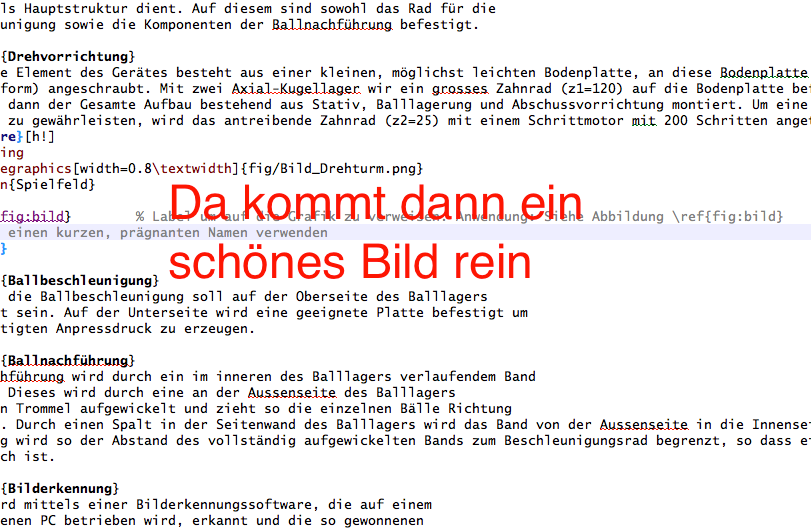
\includegraphics[width=0.8\textwidth]{fig/Bild_Drehturm.png}    
	\caption{Drehvorrichtung}
	
	\label{fig:bild}        % Label um auf die Grafik zu verweisen. Anwendung: Siehe Abbildung \ref{fig:bild}
	% Bitte einen kurzen, prägnanten Namen verwenden
\end{figure}

Um eine genaue Ausrichtung zu gewährleisten, wird das antreibende Zahnrad 
(Zähnezahl z2=25) mit einem Schrittmotor mit 200 Schritten angetrieben (Schrittmotor QSH 4218, 
QMot.eu). Bei 200 Schritten ergibt sich eine Genauigkeit von 1.8$^\circ$, mit einer 
Übersetzung von z1/z2=4.8 ergibt das eine Ausrichtgenauigkeit von 0.375$^\circ$. Dies 
bedeutet für eine Distanz von 1900mm eine seitliche Abweichung von 
$1900 \cdot \tan(0.375^\circ)= 12.5mm$. Somit wird diese Abweichung bei einem 
Korbdurchmessen von 30cm keine Rolle spielen. Des Weiteren wird mit einem 
geeigneten Treiber sogar noch eine höhere Genauigkeit erreicht 
(Zwischenschritte), welche jedoch vom Drehmoment abhängig ist. 

\subsection{Ballbeschleunigung}
Das Rad für die Ballbeschleunigung soll auf der Oberseite des Balllagers 
positioniert sein. Auf der Unterseite wird eine geeignete Platte befestigt um 
so den benötigten Anpressdruck zu erzeugen. 
Die Beschleunigung des Rads soll mittels einem integrierten brushless Motor erfolgen. Hierzu wird das Rad selbst hergestellt und die benötigten Magnete direkt in der Felge verbaut. Das Grundgerüst für den Stator kann aus einem alten Motor ausgebaut und verwendet werden. Jedoch wird die Wicklung für eine angepasste Funktionalität selbst aufgebracht.

\subsection{Ballnachführung}
Die Ballnachführung wird durch ein im Inneren des Balllagers verlaufendes Band 
realisiert. Dieses wird durch eine an der Aussenseite des Balllagers 
angebrachten Trommel aufgewickelt und zieht so die einzelnen Bälle in Richtung 
Abschussrad. Durch einen Spalt in der Seitenwand des Balllagers wird das Band 
von der Aussenseite in die Innenseite geführt. Gleichzeitig wird so der 
Abstand des vollständig aufgewickelten Bands zum Beschleunigungsrad begrenzt, 
so dass ein Verklemmen nicht möglich ist.
Die Trommel wird durch einen, mit einem Zahnriemen verbundenen Schrittmotor angetrieben.

\subsection{Bilderkennung}
Ziel der Bilderkennung ist es, zu erkennen wo sich der Korb auf der Spielfläche befindet. Das Bild muss so verarbeitet werden, dass in einem ersten Schritt der Korb erkannt wird und in einem zweiten Schritt die Position errechnet werden kann.
\subsubsection{Hardware}
Bei der Bildverarbeitung ist zu beachten, dass sie sehr rechen- wie auch speicherintensiv ist. Um eine Analyse eines Bildes durchzuführen sind diverse mathematische Funktionen wie auch farb-analytische Schritte nötig. Je schneller die Berechnung ausgeführt werden soll, desto grössere Rechenleistungen werden benötigt. Deshalb wurde entschieden, die Bildverarbeitung auf ein Notebook auszulagern. Dieses sollte neben genügend Speicher auch ausreichend Rechenleistung zu Verfügung stellen können. Da sämtliche Studierende bereits über ein Notebook verfügen, vereinfacht sich die gemeinsame Entwicklung auf dem Endgerät.

\subsubsection{Software}
Als Entwicklungssprache für die Bildverarbeitung hat sich die Gruppe, basierend auf der Technologierecherche, für Java entschieden. Dies vor allem auch weil sämtliche Elektrotechnik- und Informatikstudierende aufgrund der besuchten Module bereits Erfahrungen mit Java sammeln konnten. Doch Java ist auch bezüglich der Komptabilität und Schnittstellen mit diversen Entwicklungsumgebungen und Sprachen die erste Wahl. Die vorhandenen Entwicklungsumgebungen können dank der breiten Community durch die zahlreichen Plug-ins fast beliebig erweitert werden.
Die Technologierecherche hat ergeben, dass sich OpenCV als geeignetste Bildverarbeitungsbibliothek zeigt. Dies unter anderem auch, weil es über eine sehr grosse und auch aktive Community verfügt. Ebenfalls auf Grund der grossen Beliebtheit von OpenCV werden sehr viele Plattformen unterstützt, was uns bei der Wahl unserer Betriebssystemen, Komponenten und Entwicklungsumgebungen kaum einschränkt.

\subsection{Signalübertragung}
Die Signalübertragung befasst sich mit der Kommunikation zwischen den beteiligten Komponenten. Einerseits wird ein leichtgewichtiges Signal benötigt um den Start und das Ende der Aufgabe zu symbolisieren. Für die Übertragung des Bildes ist allerdings ein Übermittlungsstandard nötig, der auf eine grössere Bandbreite zurückgreifen kann.

\begin{figure}[h!]          
	\centering             
	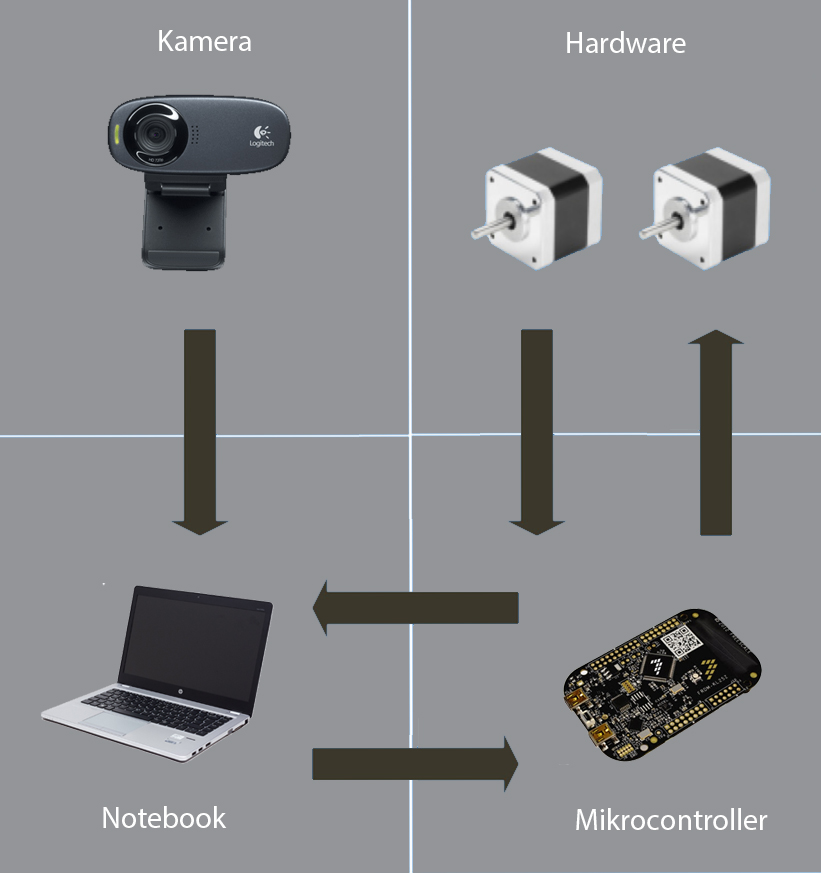
\includegraphics[width=0.5\textwidth]{fig/kommunikationsablauf.jpg}    
	\caption{Kommunikationsablauf}
	
	\label{fig:Kommunikationsablauf}
\end{figure}
\noindent
\subsubsection{Start- und Endsignal}
Das Startsignal wird drahtlos vom Laptop auf den Roboter übertragen. Nachdem dieser die Aufgabe ausgeführt hat, sendet dieser wiederum drahtlos das Endsignal an den Laptop. Aufgrund der Technologierecherche wurde entschieden, dass Bluetooth sich am besten für diese Übertragung eignet. Nach der Erweiterung durch entsprechende Module unterstützt Bluetooth sowohl Mikrocontroller als auch reguläre Computer. Die vorgegebenen Schnittstellen vereinfachen die drahtlose Kommunikation.
\subsubsection{Bildübermittlung}
Je höher die Auflösung des vorhandenen Bildes, desto genauer kann die Position vom Laptop bestimmt werden. Je höher die Auflösung, desto grösser wird die Bilddatei die zum Laptop übermittelt werden muss. Am naheliegendsten wäre die Verwendung von Bluetooth gewesen. Doch aufgrund von ungenügender Bandbreite muss auf einen anderen Übermittlungsstandard zurückgegriffen werden. Die Bildübertragung kann unabhängig vom Mikrocontroller geschehen. So kann sich dieser alleine auf die Abarbeitung des Schiessvorgangs konzentrieren. Das Bild wird separat entweder direkt von einer Kamera oder von einem weitere Mikrocontroller übermittelt. Um diese Übermittlung durchzuführen wurde WLAN ausgewählt. Dies vorallem, weil WLAN ein sehr verbreiteter Standard ist und fast von allen Geräten unterstützt wird. Zudem können im Handel preisgünstig WLAN-fähige Kameras erworben werden.

\clearpage
\section{Berechnungen}
\label{sec:calc}

\subsection{Spielfeld}
\begin{figure}[h!]          
    \centering             
    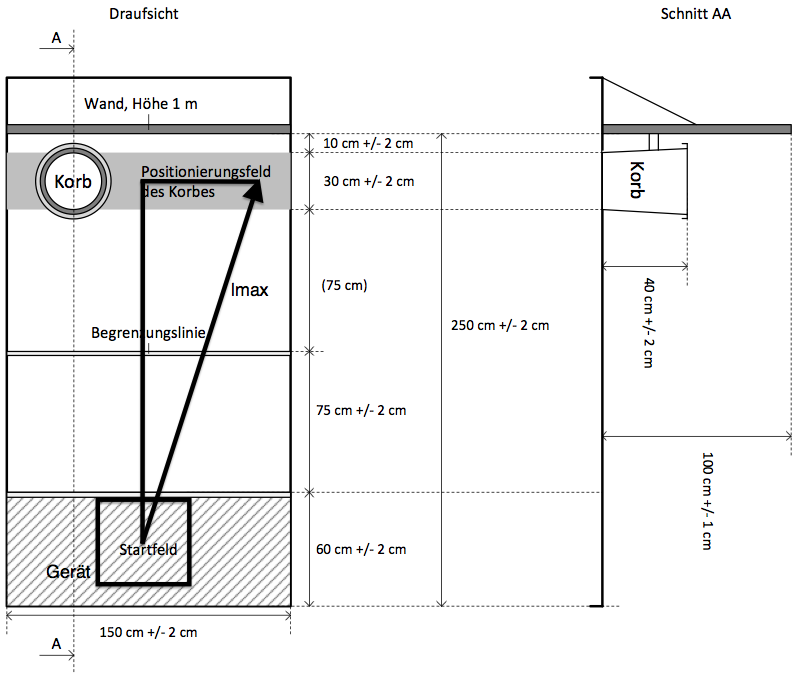
\includegraphics[width=0.8\textwidth]{fig/Bild_Spielfeld.png}    
    \caption{Spielfeld}
    \label{fig:spielfeld}        
\end{figure}
\noindent
Angenommen das Gerät wird im Startfeld mittig an der Startlinie positioniert, 
ausschliesslich mit einer drehbaren Abschussvorrichtung ausgerüstet, und der 
Korb ganz am Rand des Feldes positioniert, so ergibt sich für die maximale 
Wurflänge $l_{max}$ folgender Wert: 

\[\ l_\text{max} = \sqrt{(600mm)^2 + (1900mm)^2} = 1992.49mm \]


Somit ergibt sich im schlechtesten Fall ein Längenunterschied von  9.25 cm. 
Je nachdem wie hoch die Wurfgenauigkeit ist, können die 9.25cm in 
Anbetracht des Korbdurchmessers von 30cm vernachlässigt werden. Unter der Voraussetzung 
dass die Zielgenauigkeit sehr hoch ist, kann ein Drehturm mit immer gleicher Wurflänge 
konstruiert werden. Bei der Variante Bodenobjekt stehend (Siehe Kapitel 5.4 und Kapitel 6.) für die wir 
uns entschieden haben, kann die Wurflänge mit sehr einfachen Mitteln über die Drehzahl
eingestellt werden, somit ist keine so hohe Zielgenauigkeit nötig.

\subsection{Berechnungen Ballwurf}
Angenommen der Ball wird auf der Höhe des Korbes abgeworfen, kann mit 
folgender Formel berechnet werden, mit welcher Geschwindigkeit der Ball 
geworfen werden muss, falls er in einem Winkel $\alpha$ von 65$^\circ$ 
geworfen wird:
%
\[ v_0 
    = \sqrt{ \frac{s_x}{\sin(2 \cdot \alpha)} \cdot g } 
    = \sqrt{ \frac{1.9m}{\sin(2 \cdot 65^\circ)} \cdot 9.81 \frac{m}{s^2}} 
    = 4.93 \frac{m}{s} \]
%
Die maximale Höhe von 1.8 Metern darf nicht überschritten werden. Die Höhe 
die, der Ball erreicht lässt sich folgendermassen berechnen:
%
\[ h_\text{max} 
    = \frac{v_0^2 \cdot \sin(\alpha)^2}{2 \cdot g} 
    = \frac{4.93 \frac{m}{s}^2 \cdot \sin(65^\circ)^2}{2 \cdot 9.81 \frac{m}{s^2}} 
    = 1.018m \]
%
Die Zeit, die der Ball braucht, bis er im Korb ist, lässt sich folgendermassen 
berechnen:
%
\[ t = \frac{s_x}{v_0 \cdot \cos(\alpha)} 
    = \frac{1.9m}{4.93 \frac{m}{s} \cdot \cos(65^\circ)} = 0.911s \]
%
Nun werden die gleichen Rechnungen mit einem Winkel von 70$^\circ$ durchgeführt:
%
\[ v_0 = \sqrt{ \frac{s_x}{\sin(2\alpha)} \cdot g } 
    = \sqrt{ \frac{1.9m}{\sin(2 \cdot 70^\circ)} \cdot 9.81 \frac{m}{s^2}} 
    = 5.385 \frac{m}{s} \]

\[ h_\text{max} = \frac{v_0^2 \cdot \sin(\alpha)^2}{2 \cdot g} 
    = \frac{5.385 \frac{m}{s}^2 \cdot \sin(70^\circ)^2}{2 \cdot 9.81 \frac{m}{s^2}} 
    = 1.305m \]

\[ t = \frac{s_x}{v_0 \cdot \cos(\alpha)} 
    = \frac{1.9m}{5.385 \frac{m}{s} \cdot \cos(70^\circ)} = 1.032s \]
%
Wenn man davon ausgeht, dass es sich bei der Abschussgeschwindigkeit ein 
absoluter Fehler von $\pm$ 0.3 m/s einstellt, kann berechnet werden, mit 
welchem Winkel die Distanz mehr variiert:

\noindent
Winkel 65$^\circ$:
%
\[ s_x = \frac{(v_0 \pm \Delta v)^2 \cdot \sin(2 \cdot \alpha)}{g} 
    = \frac{(4.93 \frac{m}{s} \pm 0.3 \frac{m}{s})^2 \cdot \sin(2 \cdot 65^\circ)}{9.81 \frac{m}{s^2}} \]

\[ s_\text{xmax} = 2.136m \hspace{30mm} s_\text{xmin} = 1.674m \]
%
Winkel 70$^\circ$:
%
\[ s_x = \frac{(v_0 \pm \Delta v)^2 \cdot \sin(2 \cdot \alpha)}{g} 
    = \frac{(5.385 \frac{m}{s} \pm 0.3 \frac{m}{s})^2 \cdot \sin(2 \cdot 70^\circ)}{9.81 \frac{m}{s^2}} \]

\[ s_\text{xmax} = 2.118m \hspace{30mm} s_\text{xmin} = 1.694m \]
%
Bei einer Abschussgeschwindigkeitsänderung von lediglich $\pm$ 0.3m/s ergibt 
sich bereits eine Abweichung der Wurfweite von $\pm$ 20-25cm. Die 
Geschwindigkeit muss sehr genau eingestellt werden können und sehr konstant sein.

\noindent
Anhand dieser Berechnungen kann man auch sagen, dass die Längenänderung mit 
grösser werdendem Winkel kleiner wird. Somit wäre es besser, den Ball in einem 
grösseren Winkel zu schiessen. Allerdings muss dann der Ball schneller 
geschossen werden (mehr Energieaufwand, grösserer Rückstoss), der Weg wird 
länger und der Flug dauert länger. Die grösste Reichweite wird mit einem Abschusswinkel 
von 45$^\circ$ erreicht. Für die von uns gewählte Variante Bodenobjekt stehend (Siehe Kapitel
5.4 und Kapitel 6.) wird der Abschusswinkel voraussichtlich 50$^\circ$ betragen (Siehe Kapitel 8.1.1).

\clearpage
\section{Tests} % Tests
\begin{frame}
    \frametitle{Übersicht}
    \pause
    \begin{block}{Elektronik}
        \begin{itemize}
            \item Sensoren zur Korberkennung
            \item BLDC Treiber
        \end{itemize}
    \end{block}
    \pause
    \begin{block}{Mechanik}
        \begin{itemize}
            \item Schussvorrichtung
            \item Drehvorrichtung
        \end{itemize}
    \end{block}
    \pause
    \begin{block}{Informatik}
        \begin{itemize}
            \item Bilderkennung
        \end{itemize}
    \end{block}
\end{frame}

\begin{frame}
    \frametitle{Sensoren}
    \begin{columns}
        \pause
        \begin{column}{0.5\textwidth}
            \begin{block}{Ultraschall - HC-SR04}
                \begin{itemize}
                    \item Laufzeit Ultraschallimpuls
                    \item $D = \frac{T \cdot c_{Luft}}{2}$
                \end{itemize}
                \pause
                \begin{figure}
                    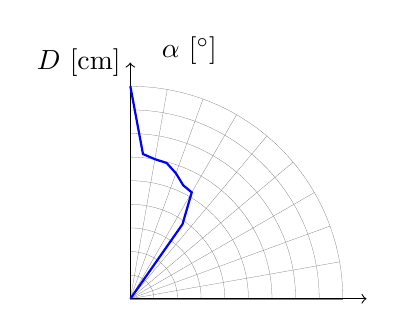
\begin{tikzpicture}[scale=1.5]
                        % Grid
                        % Grid for Angle
                        \foreach \i in {0, 10, ..., 90}
                        {
                            \draw[ultra thin, gray]
                                (90-\i:0) -- (90-\i:1.8);
                                %node[above right, black] {\i};
                        }
                        % Grid for Distance
                        \foreach \i in {0, 20, ..., 180}
                        {
                            \draw[ultra thin, gray]
                                (0.01*\i,0) arc [radius = 0.01*\i, start angle = 0, end angle = 90];
                                %node[left, black] {\i};
                        }
                        % Axis
                        \draw[->] (0:0) -- (0:2);
                        \draw[->] (0:0) -- (90:2) node[left] {$D$ [cm]};
                        \node at (0.5, 2.1) {$\alpha$ [$^\circ$]};
                        % Data
                        \draw[thick, blue]
                            (90 - 0  : 1.80) --
                            (90 - 5  : 1.23) --
                            (90 - 10 : 1.20) --
                            (90 - 15 : 1.19) --
                            (90 - 20 : 1.13) --
                            (90 - 25 : 1.06) --
                            (90 - 30 : 1.04) --
                            (90 - 35 : 0.77) --
                            (90 - 40 : 0.00) ;
                    \end{tikzpicture}
                \end{figure}
            \end{block}
        \end{column}
        \pause
        \begin{column}{0.5\textwidth}
            \begin{block}{Infrarot - GP2Y0A710K0F}
                \begin{itemize}
                    \item Triangulation
                    \item $D = d \cdot \arctan(\alpha)$
                \end{itemize}
                \pause
                \begin{figure}
                    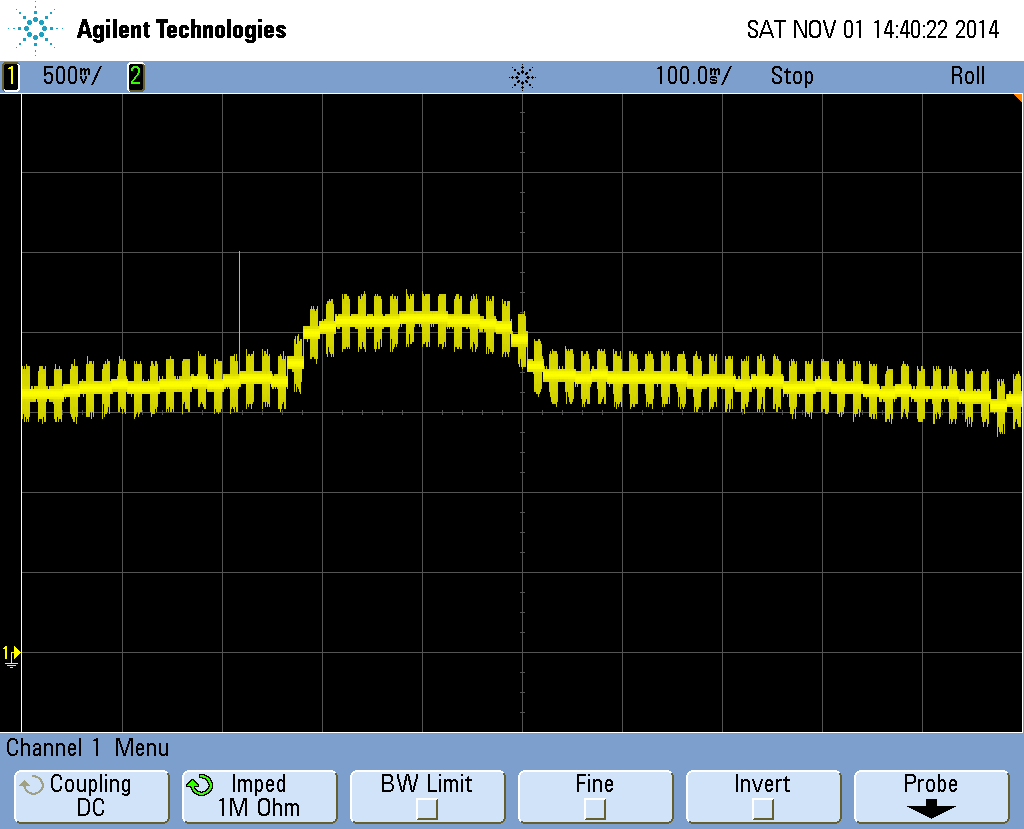
\includegraphics[width=0.8\textwidth]{../doc/fig/scope_82.png}
                \end{figure}
            \end{block}
        \end{column}
    \end{columns}
\end{frame}

\begin{frame}
    \frametitle{BLDC}
\end{frame}

\begin{frame}
    \frametitle{Schussvorrichtung}
\end{frame}

\clearpage
\section{Schlussdiskussion}

\subsection{Erfahrungen}

\subsubsection*{Daniel Mathis}
Zu Beginn war es wichtig, die Teammitglieder kennenzulernen, um so ein 
möglichst breites Vorwissen aufzubauen. Anhand dieses Vorwissens, 
konzentrierten wir uns schnell auf eine Lösung welche fliegen sollte. Die uns 
anschliessend in Auftrag gegebene Risikoanalyse zeigte jedoch auf, dass diese 
Lösung ein zu hohes Risiko darstellt. Dieses zeigte mir persönlich die 
Wichtigkeit eines strukturierten Ablaufes auf. Des weiteren war es nicht ganz 
einfach, die Aufgabenstellung zu unterteilen in die verschiedenen Teilsysteme 
und zu diesen Teilsystemen möglichst viele Möglichkeiten aufzuzeigen. 
Rückblickend betrachtend, gelang dies uns jedoch relativ gut. Eine weitere 
Schwierigkeit für mich waren die Berichte, welche abgegeben werden mussten. 
Deren Inhalt aus meiner Sicht nicht immer klar definiert war und uns daher 
etwas aus dem Zeitplan brachte. Im Grossen und Ganzen konnte ich jedoch viel 
von der Interdisziplinarität dieses Projektes profitieren und habe deshalb 
auch einiges über die Schnittstellen zwischen Mechanik und der Elektronik 
erlernt. Ich bin gespannt auf das nächste Semester, wenn wir unsere Ideen zu 
einer kompletten Maschine verbinden können.

\subsubsection*{Peter Kuonen}
Bereits im ersten Semester habe ich gute Erfahrungen mit dem Kontext-Modul erleben dürfen. Deshalb freute ich mich auf das PREN1-Modul besonders. Eine weitere Möglichkeit ein Interdisziplinäres Projekt umzusetzen. Es ist für mich immer spannend neue Menschen kennen zu lernen und die verschiedenen Fähigkeiten zu kombinieren. Beim PREN1 hatten wir wieder das Glück, dass sich die Gruppe auf Anhieb verstanden hat. Dies war für mich einer der wichtigsten Aspekte. Wenn das Team funktioniert, funktioniert auch das Projekt.\\
%
Was das Projekt selbst angeht, war ich etwas enttäuscht. Die Anfangs-Euphorie hat sich relativ bald gelegt. Die Aufgabe bestand lediglich darin Bälle in einen Korb zu versenken. Nach der Risikoanalyse stellte sich heraus, dass fliegende Lösungen keinen Sinn machen (zu viele Risiken) und dann blieb als beste Lösung ein stillstehender, sich drehender Turm. Im Bereich Informatik ist  kaum etwas zu tun. Im Vergleich zu vorhergehenden Jahren, bei der die Informatik auch einen beträchtlichen Beitrag zur Lösung leisten durfte.\\
%
Bei der Dokumentation und den Zwischenabgaben hatten wir unsere liebe Mühe. Teilweise wussten wir nicht genau was verlangt war. Nach mehreren Gesprächen mit dem Experten hat es  schlussendlich geklappt. Hier wären mir von Beginn an etwas mehr Informationen lieber gewesen. Da wir noch nie ein Projekt von diesem Umfang bearbeitet haben, ist die Führung durch die Dokumentation verloren gegangen. 
Im Grossen und Ganzen hat das PREN1 jedoch Spass gemacht und das Team hat wunderbar zusammen gearbeitet. Ich bin gespannt auf das nächste Semester, wenn wir unser Konzept zusammen im PREN2 umsetzen können.


\subsection{Offene Punkte/Risikien/Ausblick}

\clearpage
\listoffigures
\listoftables
\section*{Quellenverzeichnis}
Das Quellenverzeichnis folgt. 
%\nocite{*}
\renewcommand{\refname}{Literatur- und Quellenverzeichnis}
\bibliography{doc.bib}

